Nesta seção apresentamos a avaliação quantitativa dos modelos individuais e das abordagens de ensemble, seguindo o protocolo descrito na Seção \ref{sec:materials_methods}.

A Tabela \ref{tab:ensemble_results_expanded} resume o desempenho em termos de Kappa Quadrático Ponderado (QWK) e acurácia, acompanhados de desvio padrão e intervalos de confiança de 95\%. Entre os modelos individuais, o EfficientNet-B0 com regressão ordinal, perda focal e filtragem por entropia apresentou o melhor desempenho (QWK = 0,856). Versões mais profundas (B3 e B7) não resultaram em melhorias, sugerindo que o aumento da capacidade do modelo não trouxe benefícios sob o pipeline adotado.

Em contraste, as estratégias de ensemble superaram consistentemente os modelos isolados. O melhor desempenho foi obtido pelo ensemble baseado em média simples, alcançando QWK = 0,879, superando tanto os modelos individuais quanto outras estratégias de agregação, como média ponderada, voto majoritário e máximo. Observa-se também melhora na acurácia, indicando maior estabilidade nas predições interclasses.

Esses resultados demonstram que a combinação de múltiplos modelos por média simples não apenas suaviza variações indesejadas, mas também captura diferentes aspectos aprendidos por cada arquitetura, resultando em uma solução mais robusta para a classificação ISUP.

\begin{table}[H]
	\centering
	\caption{Comparação de desempenho: Kappa e Acurácia (com Desvio Padrão e Intervalo de Confiança).}
	\label{tab:ensemble_results_expanded}
	\resizebox{\textwidth}{!}{%
		\begin{tabular}{lcccccc}
			\toprule
			& \multicolumn{3}{c}{\textbf{Kappa}} & \multicolumn{3}{c}{\textbf{Acurácia}} \\
			\cmidrule(lr){2-4} \cmidrule(lr){5-7}
			\textbf{Model} & \textbf{Resultado} & \textbf{Std} & \textbf{IC 95\%} & \textbf{Resultado} & \textbf{Std} & \textbf{IC 95\%} \\
			\midrule
			Ensemble-Mean              & \textbf{0,879} & 0,010 & [0,858; 0,898] & \textbf{0,698} & 0,011 & [0,676; 0,721] \\
			Ensemble-Weighted          & 0,878          & 0,009 & [0,858; 0,895] & 0,692 & 0,011 & [0,669; 0,714] \\
			Ensemble-Vote              & 0,859          & 0,011 & [0,835; 0,882] & 0,692 & 0,011 & [0,668; 0,715] \\
			\midrule
			B0-Entropy-Ordinal-Focal   & 0,856          & 0,011 & [0,833; 0,876] & 0,660 & 0,012 & [0,635; 0,683] \\
			B0-Entropy-Ordinal-Focal SWA & 0,852        & 0,011 & [0,830; 0,873] & 0,653 & 0,012 & [0,629; 0,676] \\
			B3-Entropy-Ordinal-Focal   & 0,848          & 0,012 & [0,824; 0,870] & 0,660 & 0,011 & [0,638; 0,683] \\
			B7-Entropy-Ordinal-Focal   & 0,844          & 0,011 & [0,821; 0,865] & 0,602 & 0,012 & [0,578; 0,628] \\
			\midrule
			Ensemble-Max               & 0,839          & 0,011 & [0,815; 0,859] & 0,582 & 0,012 & [0,559; 0,605] \\
			B0-Baseline          & 0,826          & 0,012 & [0,806; 0,846] & 0,592 & 0,012 & [0,572; 0,612] \\
			\bottomrule
		\end{tabular}%
	}
\end{table}

As matrizes de confusão da Figura~\ref{fig:comparison_b0} mostram que o modelo B0-Baseline apresenta maior dispersão dos erros, com confusões frequentes entre classes não adjacentes, especialmente nos graus intermediários (ISUP 2–4). Isso indica que, sem a perda ordinal com focal loss, o modelo não consegue capturar adequadamente a natureza ordinal do problema.
Por outro lado, o modelo B0-Entropy-Ordinal-Focal gera uma matriz de confusão muito mais concentrada na diagonal, reduzindo erros distantes e limitando as confusões principalmente a classes vizinhas, um comportamento alinhado ao esperado clinicamente. Embora tenha sido superado apenas na categoria ISUP 0, sua maior precisão nos graus mais agressivos reforça sua relevância clínica, já que esses casos demandam diagnósticos mais consistentes e confiáveis.

\begin{figure}[H]
	\centering
	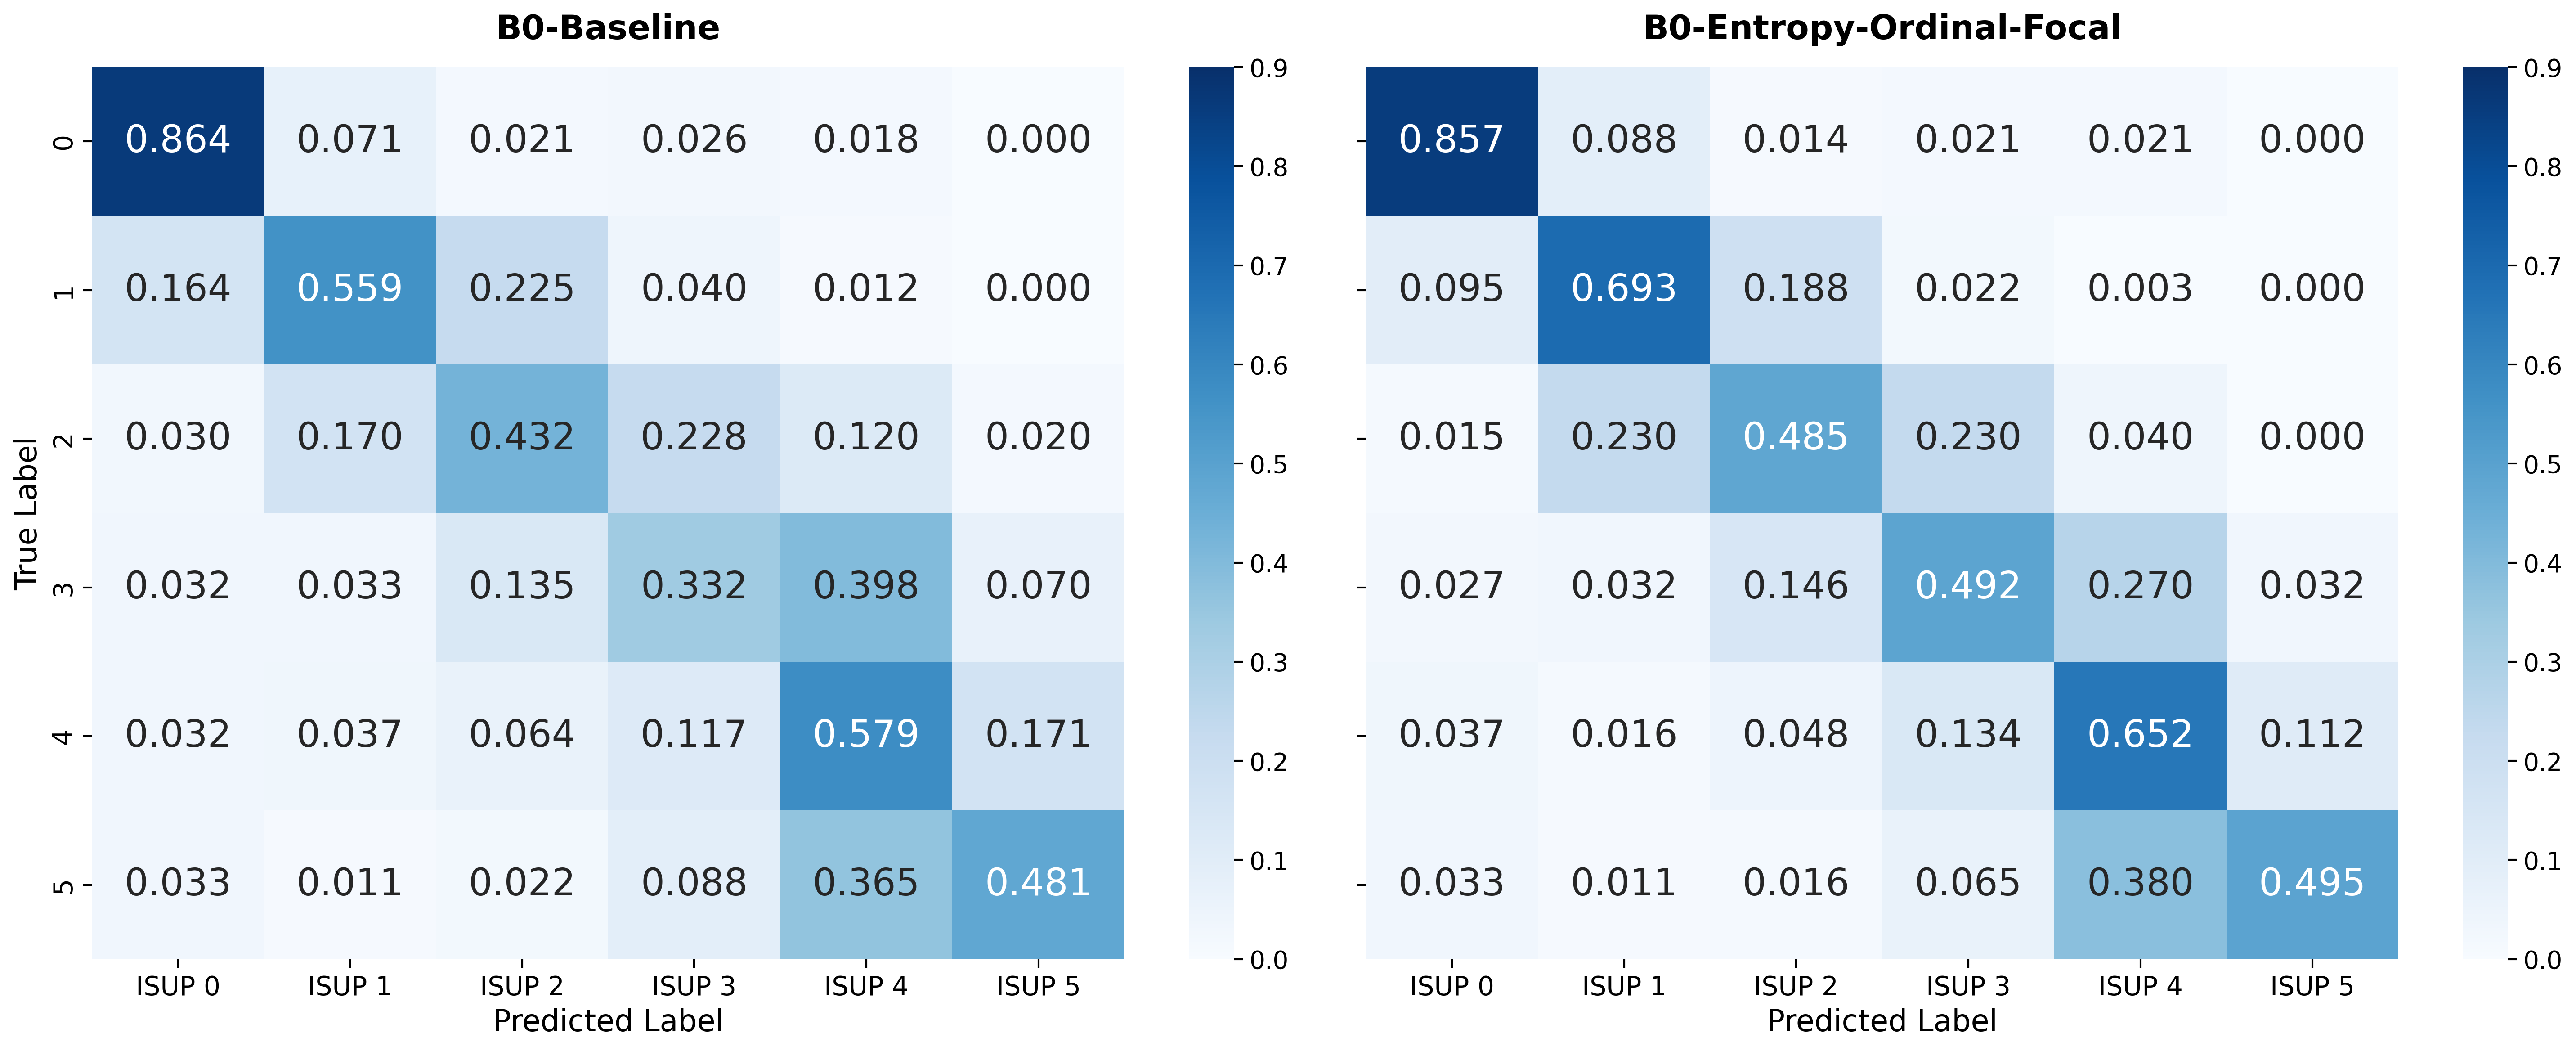
\includegraphics[width=1\linewidth]{images/comparison_cm_b0}
	\caption{Comparação entre o baseline e o melhor modelo  individual}
	\label{fig:comparison_b0}
\end{figure}

A análise da matriz de confusão do modelo Ensemble (Figura \ref{fig:ensemble}) evidencia um desempenho robusto, caracterizado pela concentração de predições na diagonal principal. O modelo demonstra alta eficácia nos casos de baixo risco (ISUP 0 e ISUP 1) e mantém consistência nos graus intermediários (ISUP 2 e 3), onde os erros se restringem majoritariamente às classes adjacentes. Nos estágios mais agressivos, a análise revela um comportamento distinto: embora a acurácia em ISUP 4 apresente uma leve retração quando comparada ao modelo B0-Entropy-Ordinal-Focal, o Ensemble compensa com uma performance superior na detecção do ISUP 5. Este resultado é particularmente relevante, pois assegura maior sensibilidade justamente no grau histológico de maior agressividade e pior prognóstico.

\begin{figure}[H]
	\centering
	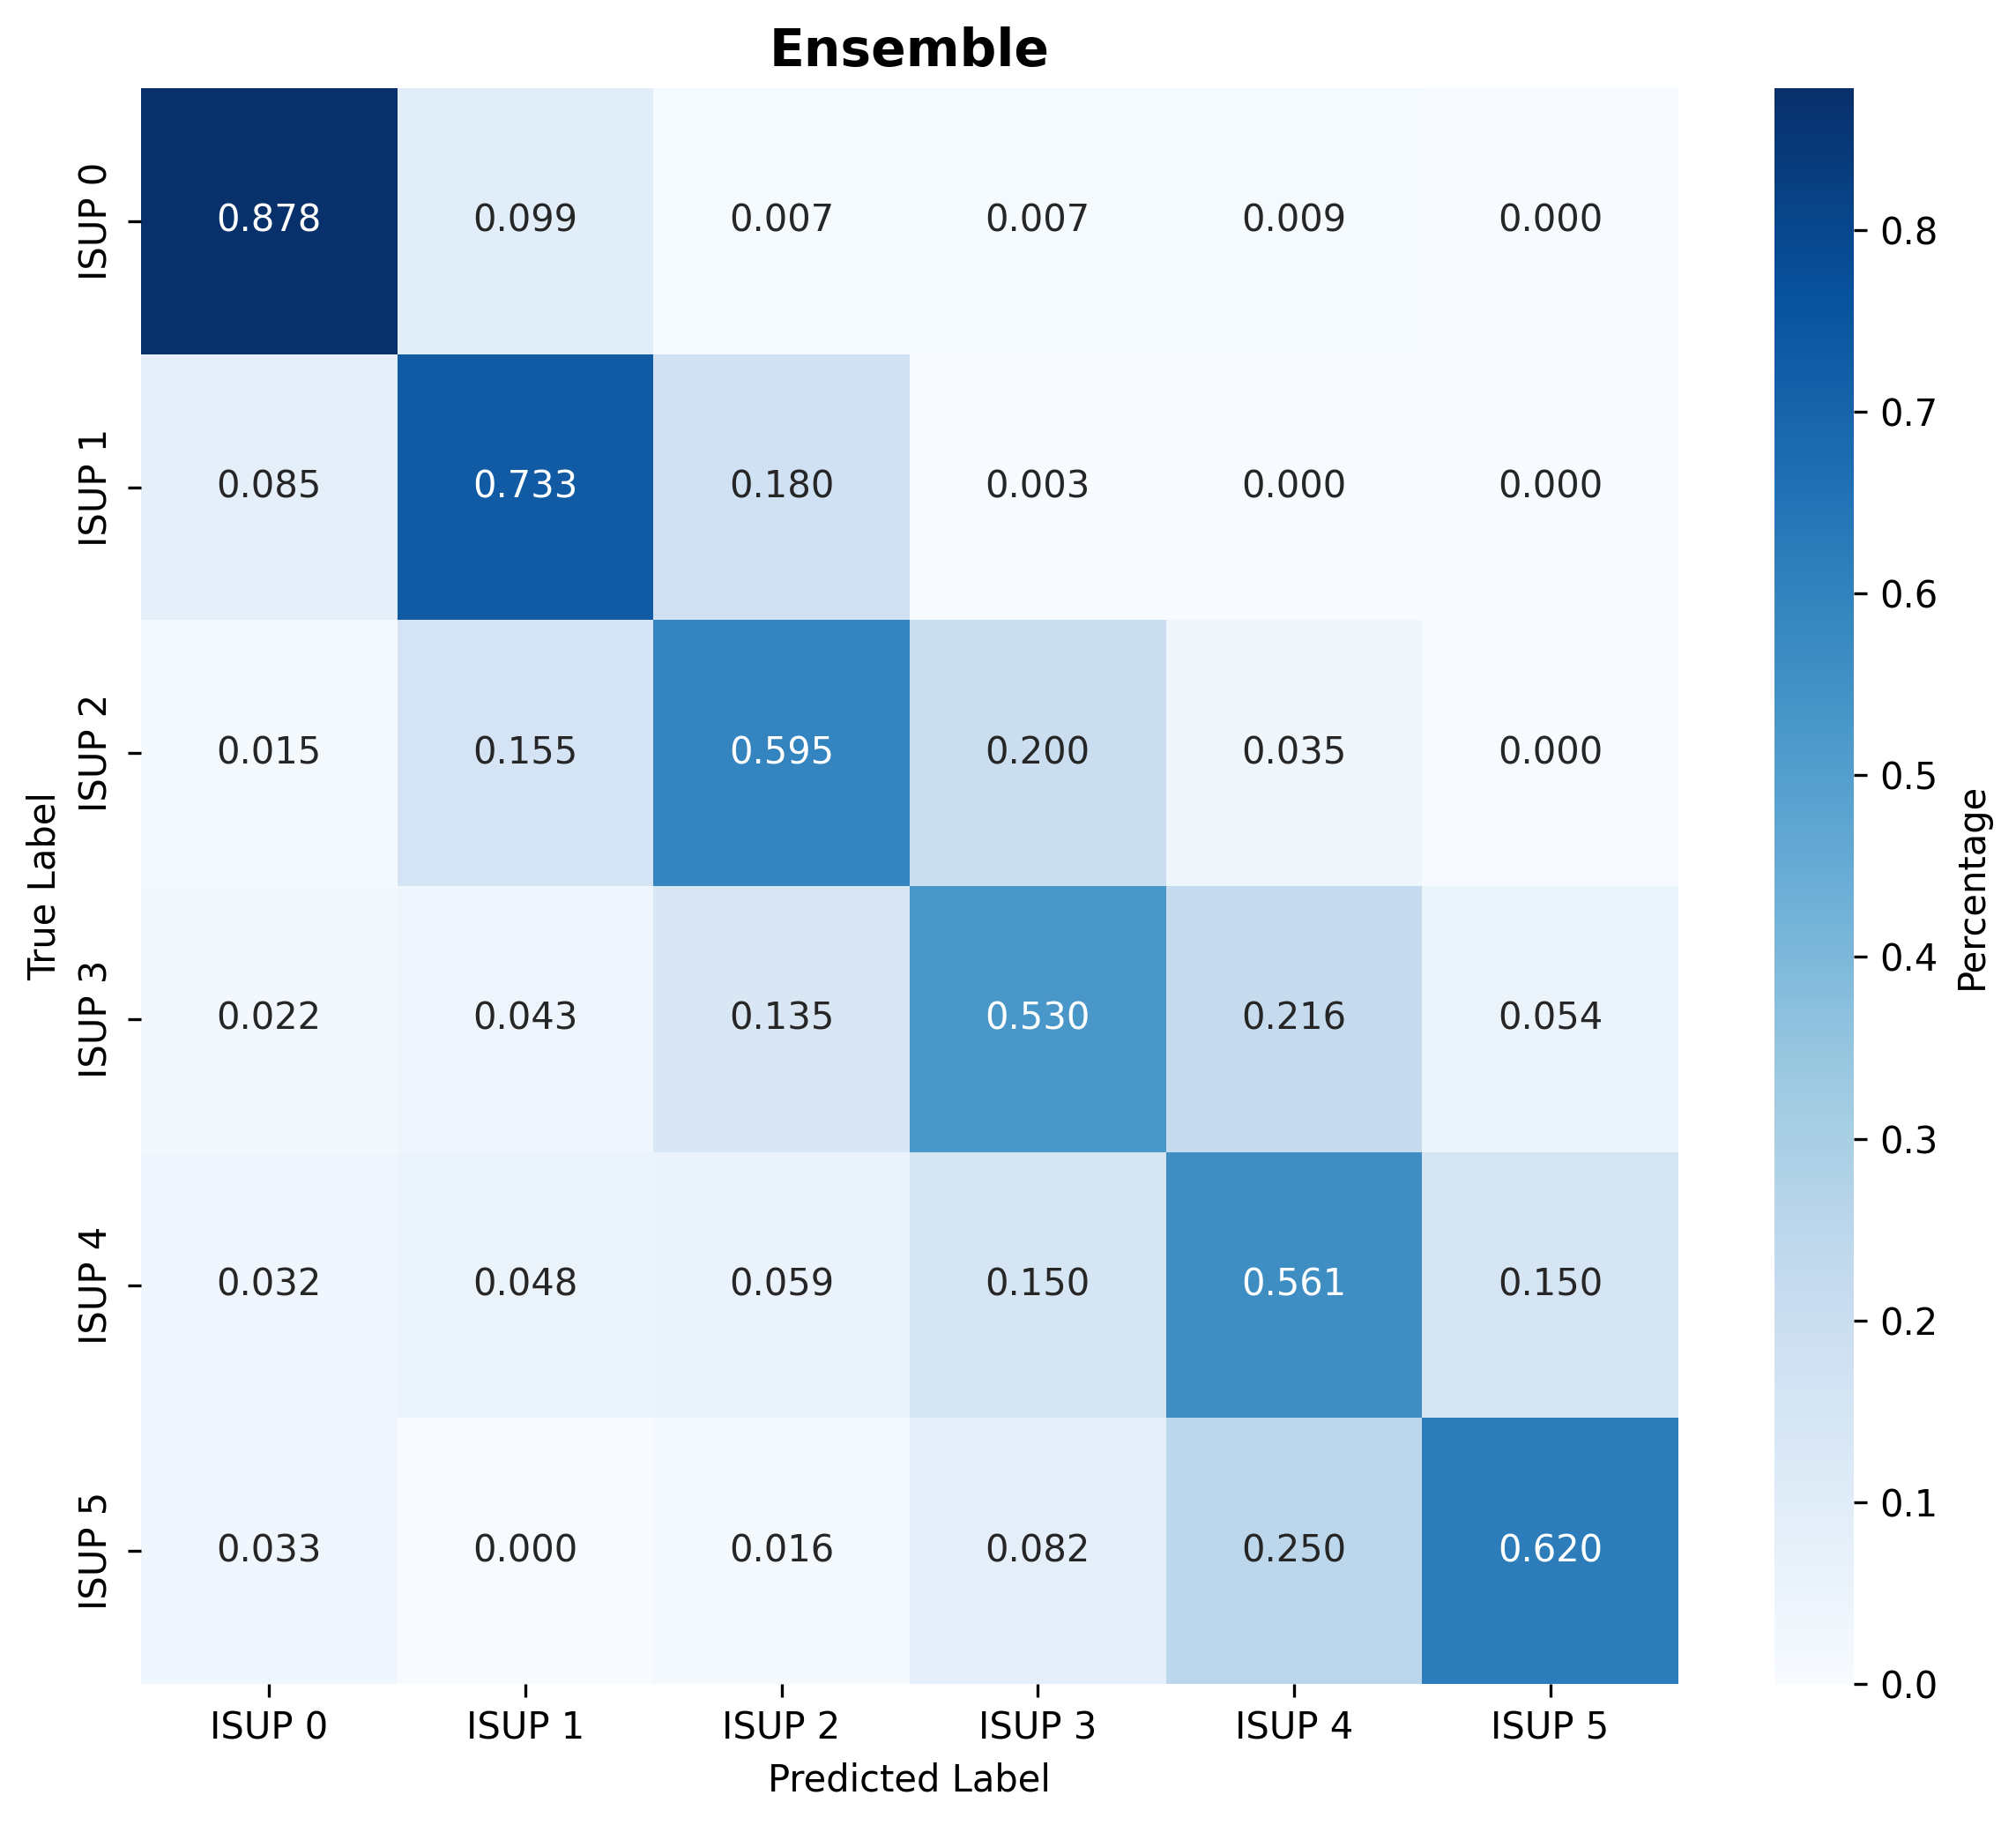
\includegraphics[width=0.8\linewidth]{images/ensemble_cm}
	\caption{Matriz de confusão do ensemble}
	\label{fig:ensemble}
\end{figure}

A Tabela \ref{tab:comparison-results} apresenta a comparação entre os resultados obtidos neste trabalho e estudos anteriores. Dada a diversidade de técnicas e bases utilizadas na literatura, destacam-se três eixos de análise: complexidade dos dados, Kappa (QWK) e consistência clínica.
\begin{itemize}
	\item \textbf{Complexidade dos dados} - Este trabalho utiliza o dataset PANDA, reconhecidamente ruidoso e com alta variabilidade institucional, um cenário que torna a tarefa mais desafiadora. Em contraste, trabalhos como os de Lucas et al. e Hammouda et al. reportam acurácias elevadas, porém com bases privadas pequenas, o que tende a inflar métricas e reduzir a capacidade de generalização.
	\item \textbf{QWK (Quadratic Weighted Kappa)} - O modelo proposto apresenta desempenho competitivo, superando estudos como Lucas et al. e Nagpal et al. Embora Singhal et al. obtenham valores superiores, esses autores utilizam arquiteturas mais pesadas e estratégias adicionais, como active learning. Neste trabalho, optou-se pela família EfficientNet, buscando um melhor equilíbrio entre desempenho e custo computacional.
	\item \textbf{Consistência clínica} - Apesar de alguns trabalhos apresentarem maior acurácia, a matriz de confusão deste estudo evidencia que o modelo preserva de forma robusta a estrutura ordinal do problema. A maioria dos erros ocorre entre classes adjacentes, alinhando-se ao comportamento clínico esperado, aspecto que métricas agregadas, como a acurácia, não capturam adequadamente.
\end{itemize}


\begin{table}[H]
	\centering
	\caption{Comparação dos resultados obtidos pelo método proposto com trabalhos relacionados do estado da arte.}
	\label{tab:comparacao_sota}
	\footnotesize % Fonte menor para melhor ajuste
	\begin{tabular}{@{}lp{2.8cm}p{2cm}p{2cm}p{3cm}@{}}
		\toprule
		\textbf{Trabalho} & \textbf{Metodologia} & \textbf{Dataset} & \textbf{Desempenho} & \textbf{Observações} \\
		\midrule
		
		\textbf{Proposto} & \textbf{Ensemble EfficientNet (B0-B3-B7) + Ordinal Focal} & \textbf{PANDA (10.616 WSIs)} & \textbf{QWK: 0,879 Acc: 69,8\%} & \textbf{Foco em redução de ruído (Entropia) e consistência ordinal.} \\
		\midrule
		
		Bulten et al.~\cite{ref-bulten2020} & U-Net Estendida & Radboud (5.759 biópsias) & QWK: 0,918 (Int.) QWK: 0,700 (Ext.) & Superou a performance de 10 entre 15 patologistas. \\
		\midrule
		
		Singhal et al.~\cite{ref-singhal2022} & U-Net + ResNeXt50 & Multicêntrico (6.670 WSIs) & QWK: 0,93 Acc: 83,1\% & Utilizou \textit{Active Learning} e adaptação de domínio. \\
		\midrule
		
		Nagpal et al.~\cite{ref-nagpal2019} & InceptionV3 + k-NN & TCGA + Outros (1.226 lâminas) & Acc: 0,70 & Superou significativamente a média de patologistas (0,61). \\
		\midrule
		
		Lucas et al.~\cite{ref-lucas2019} & InceptionV3 & Privado (96 seções) & QWK: 0,70 & Dataset limitado; alta acurácia apenas para classes binárias. \\
		\midrule
		
		Kott et al.~\cite{ref-kott2019} & ResNet-18 & Privado (85 WSIs) & Acc: 85,4\% & Estudo piloto com foco em graduação multiclasse. \\
		\midrule
		
		Hammouda et al.~\cite{ref-hammouda2021} & CNN Piramidal & Radboud (608 imagens) & Acc: 94\% & Dataset pequeno e balanceado artificialmente. \\
		
		\bottomrule
	\end{tabular}
	\label{tab:comparison-results}
\end{table}